\section{Data model and problem}
\label{sec:background}
We first define a model that maps tweet posts to documents of
different time and geographic granularities. We then review the
principles of general-purpose topic modeling with LDA~\cite{lda} and
health-related topic modeling with \atam~\cite{atam2}. We conclude this
section with our problem definition.

\subsection{Mapping Tweets to Documents}
\begin{table}[b!]
\centering
\caption{Mapping tweets to documents}
\label{tab:model:terms}
\begin{tabular}{|c|c|}
\hline
{\bf Term} & {\bf Description}\\
\hline
$\mf P$ & posts\\
\hline
$\mf G$ & regions\\
\hline
$\mf T$ & time periods\\
\hline
$\mf P_g^t$ & posts from region $g$ during time $t$\\
\hline
$D_g^t$ & document-set built by mapping the content\\
& of each post $p\in \mf P_g^t$ to a document\\
\hline
\end{tabular}
\end{table}

We consider a set of posts $\mf P=\{p_1,p_2...p_n\}$. A \emph{post} 
is the smallest unit of user-activity on a social media platform, 
such as a tweet, a tumblr post, or a facebook status update. In 
addition to a unique identifier and content, we assume the existence 
of two attributes, geographic coordinates and timestamp, for each
post, $<id,\ coord,\ tstamp,\ content>$.

Let $\mf G=\{g_1,g_2,...\}$ represent a set of geographic regions 
around the world. We use $\mf P_g$ to refer to the set of posts 
in $\mf P$ that originate from a region $g \in \mf G$. The choice 
of a geographic granularity (country, state, county) is required 
to instantiate $\mf G$.

In similar fashion, with a suitable choice of temporal granularity, 
we could divide up the entire time range spanned by posts in $\mf P$ into 
{\em disjoint and consecutive} periods, $\mf T=\{t_1,t_2...\}$. 
Possible choices for instantiation of $\mf T$ are week, bi-week, 
month, etc. We use $\mf P_g^t$ to refer to the set of posts in
$\mf P$ that originated from a region $g$ during period $t$.
% \comment{
% 	\begin{equation}
% 		\label{eq:pgt}
% 		\mf P_g^t=\{p|p\in \mf P,\ p.coord \in g,\ p.tstamp\in t\}
% 	\end{equation}
% }
We consider a set of documents $D_g^t$ formed by mapping the content 
of each post in $P_g^t$ to a document. We use 
$\mf D=\{D_g^{t_1},D_g^{t_2},\ldots\}$ to denote all document-sets 
corresponding to tweets from region $g$ for different time periods in $\mf T$.

Table~\ref{tab:model:terms} presents a summarized
version of the terminology associated to our work.

\subsection{Uncovering Latent Topics in Tweets}
We now review the principles of general-purpose topic modeling and
health-related topic modeling. Existing models are (generally)
unsupervised generative models that describe document content in a
large document collection $D$. In our case, $D$ corresponds to
$D_g^t$, the set of documents built from tweets originating from 
region $g$ during time period $t$. 

\subsubsection{Uncovering Latent Topics with LDA}
Latent Dirichlet Allocation (LDA) represents each document as
a probability distribution over $k$ topics~\cite{lda}. Each topic 
in turn $z$ is represented as a probability distribution over a set of
words. LDA assumes that the topic distribution $\theta_d$ of a 
document $d$ and the vocabulary distribution $\phi_z$ of a 
topic $z$ are generated according to a Dirichlet distribution. 
Vectorial parameters $\alpha$ and $\beta$ of the Dirichlet distribution
are assumed to be common to the corpus.

While LDA is successful at uncovering generic topics such as
``healthcare'', ``obesity'', ``substance abuse'' infrequent topics 
that may be related to specific subjects, such as the
topic ``tobacco use'', pose a challenge to LDA. Furthermore, for an
excessively frequent topic, such as ``weight loss'', LDA adds noise,
in the form of words such as ``gardening'', ``oils'', ``anti-ageing'', 
``muscle gain'', that are not related to the topic~\cite{atam2,prier2011identifying}.
Due to such limitations, LDA is not a good choice for modeling latent topics
present in health--related data.

\subsubsection{Uncovering Health Topics with \atam}
The probabilistic \emph{Ailment Topic Aspect Model} was designed 
specifically to uncover latent health-related topics present in a 
collection of tweets~\cite{atam2}. The proposed method achieves
remarkable improvement over LDA in discovering topics that correspond to 
ailments (in addition to discovering general topics). The novelty 
of \atam is that it distinguishes {\em background words} 
such as ``home'' and ``watching TV'' from {\em health-related words} 
such as ``hurts'' and ``allergy''. For each document, 
these health--related words are considered to correspond to a unique 
ailment such as ``obesity'',``insomnia'' or ``injuries''.
The word could be associated to the ailment as its symptom 
(e.g., the word ``weight'' is clearly a symptom related to the ailment
``obesity''), a treatment (the word ``diet'' is clearly a symptom
related to the ailment ``obesity'') or a general word (the word
``dentist'' is not a background word and belongs to the vocabulary of
the ailment ``dental'' but is neither a symptom nor a treatment).

% \comment{
% 	\begin{itemize}
% 	\item Set the background switching binomial $\lambda$
% 	\item Draw an ailment distribution $\eta\sim Dir(\sigma)$
% 	\item Draw word multinomials $\phi\sim Dir(\beta)$ for the topic, ailment,  and background distributions
% 	\item For each message $1 \leq m \leq D$
% 	\begin{itemize}
% 	\item Draw a switching distribution $\pi\sim Beta(\gamma_0,\gamma_1)$
% 	\item Draw an ailment $a \sim Mult(\eta)$
% 	\item Draw a topic distribution $\theta \sim Dir(\alpha_a)$
% 	\item For each word $w_i \in  N_m$
% 	\begin{itemize}
% 	\item Draw aspect $y_i\in\{0,1,2\}$ (observed)
% 	\item Draw background switcher $\ell\in\{0,1\} \sim Bi(\lambda)$
% 	\item If $\ell == 0$~: Draw $w_i \sim Mult(\phi_{B,y})$ (a background)
% 	\item Else:
% 	\begin{itemize}
% 	\item Draw $x_i \in\{0,1\}\sim Be(\pi)$
% 	\item If $x_i == 0$ (draw word from topic $z$)~:Draw topic $z_i \sim Mult(\theta)$ and word $w_i \sim Mult(\phi_z)$.
% 	\item Else: (draw word from ailment $a$, aspect $y$)~: Draw $w_i\sim Mult(\phi_{a,y})$
% 	\end{itemize}
% 	\end{itemize}
% 	\end{itemize}
% 	\end{itemize}
% }

When generating a document (tweet), one first
associates to it an ailment such as ``allergy'', ``insomnia'' or
``injury''. Thereafter, the document is generated word by
word. Using the random variables $\ell$ and $x$, one chooses if the
word is a background word or a general-purpose word ($\ell=0$ or $\ell=1,x=0$). The word can be
drawn from a vocabulary distribution common to the whole corpus (case
$\ell=0$) or generated from a LDA-type (from an underlying Dirichlet distribution)
 topic $z$ (case $\ell=1,x=0$). When the
word is related to health (case $\ell=1,x=1$), the random variable $y$
enables to choose if this word is a aspect-neutral (case $y=0$), a
symptom (case $y=1$) or a treatment (case $y=2$). Words are hence
drawn depending on the ailment $a$ which has been associated to the
document. The topic distribution vector for a sample tweet is shown 
in Figure~\ref{fig:ldavsatam}. Note the stronger relevance to 
health--related matters in this vector than in the topic distribution vector 
generated by LDA for the same tweet. 
\begin{figure}[t!]
\centering
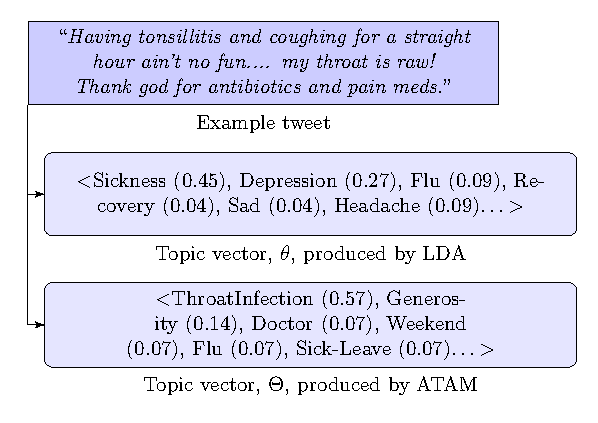
\includegraphics[width=0.45\textwidth]{tikz/exampleTweet1.pdf}
\caption{\lda vs \atam: Comparison of topic distributions for an example tweet.}
\label{fig:ldavsatam}
\end{figure}

\subsubsection{Topic Evolution Over Time}
\begin{figure}[b!]
\centering
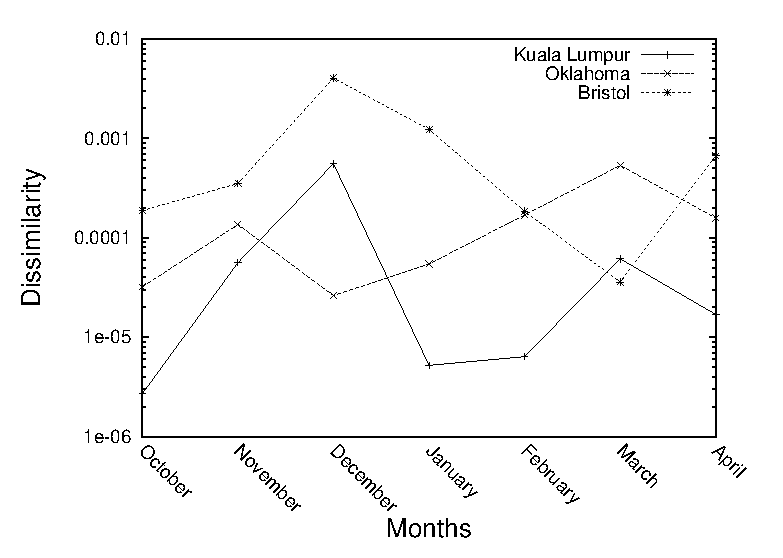
\includegraphics[width=0.45\textwidth]{gnuplot/distributiondifference/bhattacharyadistance.eps}
\caption{Topic transitions over time.}
\label{fig:ailmentsEvolve}
\end{figure}

We convert inferences of \atam over a single document to associate with a given set of documents $D_g^t$, an ailment
distribution, $\Theta_g^t$. $\Theta_g^t$ is a mix of general-purpose and health-related topics.
 $\Theta_g^t$ is a vector over a set of latent ailments where the weight of each ailment is representative of 
the ailment's occurrence in the tweets originating from region $g$ 
during period $t$. 


Ailment distributions evolve over time. Further the evolution is
region-specific as the spread of ailments is heavily influenced by the
weather and by socio-economic factors. For a region $g$, the interval
of time spanning a set of consecutive time periods
$\{t_i,t_{i+1},\ldots\}$ during which discovered ailment distributions 
$\{\Theta_g^{t_i},\Theta_g^{t_{i+1}},\ldots\}$
do not change appreciably forms a \texttt{\emph{\season}} w.r.t. ailments. By definition, a \season is (nearly) homogeneous in terms
of ailments. In other words, the ailments evolve in a smooth fashion
within a \season and change abruptly across \season boundary. We posit that such \seasons exist after which they encounter \changes in ailment topic discussions.
These \changes in ailment topic discussions 
may be caused by onset of the disease or some other external factors.
Nevertheless, they are the interesting points for analyzing purposes.

As an example, in Figure~\ref{fig:ailmentsEvolve}, we show the difference
between ailment distributions of consecutive months for 3 different
regions Kuala Lumpur (a city in Indonesia), Oklahoma (a state in
the USA), and Bristol (a city in the UK). The sharp peaks obtained
validate the existence of time intervals that are homogeneous w.r.t. ailments.

Note that a high weight for ailment $a$ in the distribution $\Theta$
only indicates that people tend to tweet about $a$ 
and need not necessarily imply
that people suffer from $a$. High weight can be attributed to a number 
of factors. For example, if a health awareness campaign on Amyotrophic 
Lateral Sclerosis 
(ALS)~\footnote{\url{https://en.wikipedia.org/wiki/Amyotrophic_lateral_sclerosis}} 
is organized in region $g$ during period $t_i$, the 
weight of ALS in $\Theta_g^{t_i}$ would be significantly higher than 
in $\Theta_g^{t_{i-1}}$ or $\Theta_g^{t_{i+1}}$ as the ailment would
appear more frequently in the tweets during period $t_i$. 
%% \begin{figure}[htpb]
%% \centering
%% \includegraphics[width=0.4\textwidth]{tikz/model.pdf}
%% \caption{\tmatam work model.}
%% \label{fig:model:tmatam}
%% \end{figure}

\subsection{Ailment prediction problem}
\label{subsec:problem-general}
We are now ready to define our problem in its general form. A more
precise form of this problem will be given in Section~\ref{subsec:problem}. 
Given a set of documents $D_g^{t_{i-1}}$ formed by tweets originating 
from a region $g \in G$ during time period $t_{i-1}$, predict the 
topic distribution of documents in $D_g^{t_i}$, corresponding to 
posts from $g$ in period $t_i$ from the topic distribution of 
document $D_g^{t_{i-1}}$ corresponding to posts from $g$ during 
period $t_{i-1}$.

Note that this problem statement does not distinguish between
general-purpose topics and health-related topics.
